\documentclass[12pt,
bibtotoc,liststotoc,appendixprefix
twoside,paper=a4,headings=small]{scrbook}
%
% Packages
% -----------------------------------
\usepackage[
  paper=a4paper,
  left=12.5mm,
  right=25mm,
  top=25mm,
  bottom=50mm,
  bindingoffset=10mm]{geometry}		% page and binding margins can be adjust here
  
\usepackage{apacite} 				% % literature-References: American Psycholog. Assoc.
\usepackage{natbib}					

\setcitestyle{round,aysep={}} 		% indexation in (round) parentheses, between the author year
\usepackage[latin1]{inputenc} 		% mutated vowel (Umlaute) in the text
\usepackage[english]{babel}				% orthography
\usepackage[T1]{fontenc}
\usepackage{lmodern}				% font family
\usepackage{microtype}				% for micro typography (for a better typeface)

\usepackage{graphicx} 				% for including graphs (pdf,png - but do avoid jpg)
\graphicspath{{./Bilder/}}          % path to the pictures

\usepackage{url}					%  formatting URL (e.g. in the literature) 
\usepackage[colorlinks,linkcolor=black,citecolor=black,urlcolor=black]{hyperref} 				% For hperlinks in PDF-documents   
  
\usepackage{tabularx} 				% for a better configuration of tables
\usepackage{longtable} 		
\usepackage{multicol}				
\usepackage{multirow}
\usepackage{booktabs}
\usepackage{tabularx}
		
\usepackage[active]{srcltx}

\usepackage{listings}				% algorithm

\usepackage{mdwlist}				% lists

\usepackage{setspace} 				% setting of the lines (rows)
\newtheorem{mydef}{Merksatz}  		% if examples or mnemotechnic verses are used with continuous numeration 
\newtheorem{bsp}{Beispiel}

\usepackage{todonotes}				% for the creation of ToDos in the editor

\usepackage{lscape}					% for the rotation of pages

\usepackage{amsmath}				% for the writting of mathematical formula

\usepackage{calc}

\usepackage{footnote}				% footnotes
\usepackage{tablefootnote}			% footnotes in tables

%\clubpenalty = 10000
%\widowpenalty = 10000 \displaywidowpenalty = 10000

\hyphenation{voll-st\"andigen}		% for defining word devisions globally

\setcounter{tocdepth}{1}			% levels which are displayed in the table of contents


% Document
% -----------------------------------
\begin{document}

\frontmatter 
    % Title page shall not include header or foooter lines
\thispagestyle{empty}

% All elements shall be centered
\begin{center}

\vspace*{-10mm}

{\LARGE CHAIR OF\\MACROECONOMICS\\[1mm]}
DER FREIEN UNIVERSIT�T BERLIN\\

\vspace*{1cm}


\includegraphics[width=0.18\textwidth]{fu_logo}

\vspace*{1cm}

% Kind of Thesis => (Bachelor Thesis ,Diploma Thesis, Master Thesis, Seminar Thesis)
{\Large \textbf{Seminar Paper in `Recent Research in Macroeconomics'}}\\ 

\vspace{1cm}

% Title of the Thesis
{\Large \textbf{Analyzing `A Behavioral New Keynesian Model'}}\\ 
\vspace*{1mm}
{\Large \textbf{by Xavier Gabaix}}\\ 


\vspace{1.5cm}

% Name of Author
{\LARGE Carlos Montoya, Patrick Molligo, and Clemens Stiewe}\\[15mm]

% Superverisor, contact data and submission date
\parbox{120mm}{
\begin{large}
\begin{tabbing}
Supervisor: \hspace{1.8cm} \=Prof. Dr. Mathias Trabandt\\[1.5mm]
Semester:\> Winter Term 2016/17\\[1.5mm]
Submission:\> 17. March 2017\\[1.5mm]
\end{tabbing}
\end{large}
}

\end{center}
\clearpage{\pagestyle{empty}\cleardoublepage}
 			% title
    \newpage
    \clearpage{\pagestyle{empty}\cleardoublepage}
        \onehalfspacing                  	% line spacing which is set to 1.5 from this point on
    \tableofcontents 					% table of contents
    \clearpage{\pagestyle{empty}\cleardoublepage} 
    
    \listoffigures 					 	% list of figures
    \clearpage{\pagestyle{empty}\cleardoublepage}
    
    \listoftables						% list of tables
    \clearpage{\pagestyle{empty}\cleardoublepage}
% -----------------------------------
\mainmatter 							% the respective chapters
    \chapter{Introduction}

Vestibulum fringilla pede sit amet augue. In turpis. Pellentesque posuere. Praesent turpis. Aenean posuere, tortor sed cursus feugiat, nunc augue blandit nunc, eu sollicitudin urna dolor sagittis lacus. Donec elit libero, sodales nec, volutpat a, suscipit non, turpis. Nullam sagittis. Suspendisse pulvinar, augue ac venenatis condimentum, sem libero volutpat nibh, nec pellentesque velit pede quis nunc. Vestibulum ante ipsum primis in faucibus orci luctus et ultrices posuere cubilia Curae; Fusce id purus. Ut varius tincidunt libero. Phasellus dolor. Maecenas vestibulum mollis diam. Pellentesque ut neque. Pellentesque habitant morbi tristique senectus et netus et malesuada fames ac turpis egestas. In dui magna, posuere eget, vestibulum et, tempor auctor, justo. In ac felis quis tortor malesuada pretium. Pellentesque auctor neque nec urna. Proin sapien ipsum, porta a, auctor quis, euismod ut, mi. Aenean viverra rhoncus pede. Pellentesque habitant morbi tristique senectus et netus et malesuada fames ac turpis egestas. Ut non enim eleifend felis pretium feugiat. Vivamus quis mi. Phasellus a est. Phasellus magna. In hac habitasse platea dictumst. Curabitur at lacus ac velit ornare lobortis. Curabitur a felis in nunc fringilla tristique.




\section{...}

Vestibulum fringilla pede sit amet augue. In turpis. Pellentesque posuere. Praesent turpis. Aenean posuere, tortor sed cursus feugiat, nunc augue blandit nunc, eu sollicitudin urna dolor sagittis lacus. Donec elit libero, sodales nec, volutpat a, suscipit non, turpis. Nullam sagittis. Suspendisse pulvinar, augue ac venenatis condimentum, sem libero volutpat nibh, nec pellentesque velit pede quis nunc. Vestibulum ante ipsum primis in faucibus orci luctus et ultrices posuere cubilia Curae; Fusce id purus. Ut varius tincidunt libero. Phasellus dolor. Maecenas vestibulum mollis diam. Pellentesque ut neque. Pellentesque habitant morbi tristique senectus et netus et malesuada fames ac turpis egestas. In dui magna, posuere eget, vestibulum et, tempor auctor, justo. 
\begin{figure}
	\centering
		
\includegraphics[width=0.7\textwidth]{./Bilder/bsp1.png}
	\caption{Beispiel 1 zum Einf�gen einer Grafik}
	\label{fig:bsp1}
\end{figure}

In ac felis quis tortor malesuada pretium. Pellentesque auctor neque nec urna. Proin sapien ipsum, porta a, auctor quis, euismod ut, mi. Aenean viverra rhoncus pede. Pellentesque habitant morbi tristique senectus et netus et malesuada fames ac turpis egestas. Ut non enim eleifend felis pretium feugiat. Vivamus quis mi. Phasellus a est. Phasellus magna. In hac habitasse platea dictumst. Curabitur at lacus ac velit ornare lobortis. Curabitur a felis in nunc fringilla tristique. 

\section{...}

Vestibulum fringilla pede sit amet augue. In turpis. Pellentesque posuere. Praesent turpis. Aenean posuere, tortor sed cursus feugiat, nunc augue blandit nunc, eu sollicitudin urna dolor sagittis lacus. Donec elit libero, sodales nec, volutpat a, suscipit non, turpis. Nullam sagittis. Suspendisse pulvinar, augue ac venenatis condimentum, sem libero volutpat nibh, nec pellentesque velit pede quis nunc. Vestibulum ante ipsum primis in faucibus orci luctus et ultrices posuere cubilia Curae; Fusce id purus. Ut varius tincidunt libero. Phasellus dolor. Maecenas vestibulum mollis diam. Pellentesque ut neque. Pellentesque habitant morbi tristique senectus et netus et malesuada fames ac turpis egestas. In dui magna, posuere eget, vestibulum et, tempor auctor, justo. In ac felis quis tortor malesuada pretium. Pellentesque auctor neque nec urna. Proin sapien ipsum, porta a, auctor quis, euismod ut, mi. Aenean viverra rhoncus pede. Pellentesque habitant morbi tristique senectus et netus et malesuada fames ac turpis egestas. Ut non enim eleifend felis pretium feugiat. Vivamus quis mi. Phasellus a est. Phasellus magna. In hac habitasse platea dictumst. Curabitur at lacus ac velit ornare lobortis. Curabitur a felis in nunc fringilla tristique.

\section{...}

Vestibulum fringilla pede sit amet augue. In turpis. Pellentesque posuere. Praesent turpis. Aenean posuere, tortor sed cursus feugiat, nunc augue blandit nunc, eu sollicitudin urna dolor sagittis lacus. Donec elit libero, sodales nec, volutpat a, suscipit non, turpis. Nullam sagittis. Suspendisse pulvinar, augue ac venenatis condimentum, sem libero volutpat nibh, nec pellentesque velit pede quis nunc. Vestibulum ante ipsum primis in faucibus orci luctus et ultrices posuere cubilia Curae; Fusce id purus. Ut varius tincidunt libero. Phasellus dolor. Maecenas vestibulum mollis diam. Pellentesque ut neque. Pellentesque habitant morbi tristique senectus et netus et malesuada fames ac turpis egestas. In dui magna, posuere eget, vestibulum et, tempor auctor, justo. In ac felis quis tortor malesuada pretium. Pellentesque auctor neque nec urna. Proin sapien ipsum, porta a, auctor quis, euismod ut, mi. Aenean viverra rhoncus pede. Pellentesque habitant morbi tristique senectus et netus et malesuada fames ac turpis egestas. Ut non enim eleifend felis pretium feugiat. Vivamus quis mi. Phasellus a est. Phasellus magna. In hac habitasse platea dictumst. Curabitur at lacus ac velit ornare lobortis. Curabitur a felis in nunc fringilla tristique. 


    \clearpage{\pagestyle{empty}\cleardoublepage}		% delets header lines and page numerbing on the last page of a chapter as long as there is no text anymore
    \chapter{Background and Literature}

Phasellus ullamcorper ipsum rutrum nunc. Nunc nonummy metus. Vestibulum volutpat pretium libero. Cras id dui. Aenean ut eros et nisl sagittis vestibulum. Nullam nulla eros, ultricies sit amet, nonummy id, imperdiet \cite{johnson1993get} feugiat, pede. Sed lectus. Donec mollis hendrerit risus. Phasellus nec sem in justo pellentesque facilisis. Etiam imperdiet imperdiet orci. Nunc nec neque. Phasellus leo dolor, tempus non, auctor et, hendrerit quis, nisi. Curabitur ligula sapien, tincidunt non, euismod vitae, posuere imperdiet, leo. Maecenas malesuada. Praesent congue erat at massa. Sed cursus turpis vitae tortor. Donec posuere vulputate arcu. Phasellus accumsan cursus velit. Vestibulum ante ipsum primis in faucibus orci luctus et ultrices posuere cubilia Curae; Sed aliquam, nisi quis porttitor congue, elit erat euismod orci, ac placerat dolor lectus quis orci. Phasellus consectetuer vestibulum elit. Aenean tellus metus, bibendum sed, posuere ac, mattis non, nunc.


\section{...}

Lorem ipsum dolor sit amet, consectetuer adipiscing elit. Aenean commodo ligula eget dolor. Aenean massa. Cum sociis natoque penatibus et magnis dis parturient montes, nascetur ridiculus mus. Donec quam felis, ultricies nec, pellentesque eu, pretium quis, sem. Nulla consequat massa quis enim. Donec pede justo, fringilla vel, aliquet nec, vulputate eget, arcu. In enim justo, rhoncus ut, imperdiet a, venenatis vitae, justo. Nullam dictum felis eu pede mollis pretium. Integer tincidunt. Cras dapibus. Vivamus elementum semper nisi. Aenean vulputate eleifend tellus. Aenean leo ligula, porttitor eu, consequat vitae, eleifend ac, enim. Aliquam lorem ante, dapibus in, viverra quis, feugiat a, tellus. Phasellus viverra nulla ut metus varius laoreet. Quisque rutrum. Aenean imperdiet. Etiam ultricies nisi vel augue. Curabitur ullamcorper ultricies nisi. Nam eget dui. Etiam rhoncus. Maecenas tempus, tellus eget condimentum rhoncus, sem quam semper \cite{kliewer2005optimierung} libero, sit amet adipiscing sem neque sed ipsum. Nam quam nunc, blandit vel, luctus pulvinar, hendrerit id, lorem. Maecenas nec odio et ante tincidunt tempus. Donec vitae sapien ut libero venenatis faucibus. Nullam quis ante. Etiam sit amet orci eget eros faucibus tincidunt. Duis leo. Sed fringilla mauris sit amet nibh. Donec sodales sagittis magna. Sed consequat, leo eget bibendum sodales, augue velit cursus nunc, quis gravida magna mi a libero. Fusce vulputate eleifend sapien. Vestibulum purus quam, scelerisque ut, mollis sed, nonummy id, metus. Nullam accumsan lorem in dui. Cras ultricies mi eu turpis hendrerit fringilla. Vestibulum ante ipsum primis in faucibus orci luctus et ultrices posuere cubilia Curae; In ac dui quis mi consectetuer lacinia. Nam pretium turpis et arcu. Duis arcu tortor, suscipit eget, imperdiet nec, imperdiet iaculis, ipsum. Sed aliquam ultrices mauris. Integer ante arcu, accumsan a, consectetuer eget, posuere ut, mauris. Praesent adipiscing. Phasellus ullamcorper ipsum rutrum nunc. Nunc nonummy metus.

\subsection{...}

Vestibulum volutpat pretium libero. Cras id dui. Aenean ut eros et nisl sagittis vestibulum. Nullam nulla eros, ultricies sit amet, nonummy id, imperdiet feugiat, pede. Sed lectus. Donec mollis hendrerit risus. Phasellus nec sem in justo pellentesque facilisis. Etiam imperdiet imperdiet orci. Nunc nec neque. Phasellus leo dolor, tempus non, auctor et, hendrerit quis, nisi. Curabitur ligula sapien, tincidunt non, euismod vitae, posuere imperdiet, leo. Maecenas malesuada. Praesent congue erat at massa. Sed cursus turpis vitae tortor. Donec posuere vulputate arcu. Phasellus accumsan cursus velit. Vestibulum ante ipsum primis in faucibus orci luctus et ultrices posuere cubilia Curae; Sed aliquam, nisi quis porttitor congue, elit erat euismod orci, ac placerat dolor lectus quis orci. Phasellus consectetuer vestibulum elit. Aenean tellus metus, bibendum sed, posuere ac, mattis non, nunc. Vestibulum fringilla pede sit amet augue. In turpis. Pellentesque posuere. Praesent turpis. Aenean posuere, tortor sed cursus feugiat, nunc augue blandit nunc, eu sollicitudin urna dolor sagittis lacus. Donec elit libero, sodales nec, volutpat a, suscipit non, turpis \cite{Fiig2004t}. Nullam sagittis. Suspendisse pulvinar, augue ac venenatis condimentum, sem libero volutpat nibh, nec pellentesque velit pede quis nunc. Vestibulum ante ipsum primis in faucibus orci luctus et ultrices posuere cubilia Curae; Fusce id purus. Ut varius tincidunt libero. Phasellus dolor. Maecenas vestibulum mollis diam. Pellentesque ut neque. Pellentesque habitant morbi tristique senectus et netus et malesuada fames ac turpis egestas. In dui magna, posuere eget, vestibulum et, tempor auctor, justo. In ac felis quis tortor malesuada pretium. Pellentesque auctor neque nec urna. Proin sapien ipsum, porta a, auctor quis, euismod ut, mi. Aenean viverra rhoncus pede. Pellentesque habitant morbi tristique senectus et netus et malesuada fames ac turpis egestas. Ut non enim eleifend felis pretium feugiat. Vivamus quis mi. Phasellus a est. Phasellus magna. In hac habitasse platea dictumst. Curabitur at lacus ac velit ornare lobortis. Curabitur a felis in nunc fringilla tristique (...)
\begin{table}[bp]
	\centering
		\caption{Beispiel 1 zum Einf�gen einer Tabelle}
		\begin{tabular}{| c c c |}
		\hline
			&&\\
			Monat & Linie & Minuten\\
			\hline
			\hline
			&&\\
			Jan & U7 & 10 \\
			Feb & U9 & 12 \\
			M�r & U9 & 20 \\
			\hline
		\end{tabular}

	\label{tab:Beispiel1}
\end{table}

\subsection{...}

 Sed cursus turpis vitae tortor. Donec posuere vulputate arcu. Phasellus accumsan cursus velit. Vestibulum ante ipsum primis in faucibus orci luctus et ultrices posuere cubilia Curae; Sed aliquam, nisi quis porttitor congue, elit erat euismod orci, ac placerat dolor lectus quis orci. Phasellus consectetuer vestibulum elit. Aenean tellus metus, bibendum sed, posuere ac, mattis non, nunc. Vestibulum fringilla pede sit amet augue. In turpis. Pellentesque posuere. Praesent turpis. Aenean posuere, tortor sed cursus feugiat, nunc augue blandit nunc, eu sollicitudin urna dolor sagittis lacus. Donec elit libero, sodales nec, volutpat a, suscipit non, turpis. Nullam sagittis. Suspendisse pulvinar, augue ac venenatis condimentum, sem libero volutpat nibh, nec pellentesque velit pede quis nunc. Vestibulum ante ipsum primis in faucibus orci luctus et ultrices posuere cubilia Curae; Fusce id purus. Ut varius tincidunt libero. Phasellus dolor. Maecenas vestibulum mollis diam. Pellentesque ut neque. Pellentesque habitant morbi tristique senectus et netus et malesuada fames ac turpis egestas. In dui magna, posuere eget, vestibulum et, tempor auctor, justo. In ac felis quis tortor malesuada pretium. Pellentesque auctor neque nec urna. Proin sapien ipsum, porta a, auctor quis, euismod ut, mi. Aenean viverra rhoncus pede. Pellentesque habitant morbi tristique senectus et netus et malesuada fames ac turpis egestas. Ut non enim eleifend felis pretium feugiat. Vivamus quis mi. Phasellus a est. Phasellus magna. In hac habitasse platea dictumst. Curabitur at lacus ac velit ornare lobortis. Curabitur a felis in nunc fringilla tristique. Vestibulum volutpat pretium libero. Cras id dui. Aenean ut eros et nisl sagittis vestibulum. Nullam nulla eros, ultricies sit amet, nonummy id, imperdiet feugiat, pede (...)

\section{...}

Lorem ipsum dolor sit amet, consectetuer adipiscing elit. Aenean commodo ligula eget dolor. Aenean massa. Cum sociis natoque penatibus et magnis dis parturient montes, nascetur ridiculus mus. Donec quam felis, ultricies nec, pellentesque eu, pretium quis, sem. Nulla consequat massa quis enim. Donec pede justo, fringilla vel, aliquet nec, vulputate eget, arcu. In enim justo, rhoncus ut, imperdiet a, venenatis vitae, justo. Nullam dictum felis eu pede mollis pretium. Integer tincidunt. Cras dapibus. Vivamus elementum semper nisi. Aenean vulputate eleifend tellus. Aenean leo ligula, porttitor eu, consequat vitae, eleifend ac, enim. Aliquam lorem ante, dapibus in, viverra quis, feugiat a, tellus. Phasellus viverra nulla ut metus varius laoreet. Quisque rutrum. Aenean imperdiet. Etiam ultricies nisi vel augue. Curabitur ullamcorper ultricies nisi. Nam eget dui. Etiam rhoncus. Maecenas tempus, tellus eget condimentum rhoncus, sem quam semper libero, sit amet adipiscing sem neque sed ipsum. Nam quam nunc, blandit vel, luctus pulvinar, hendrerit id, lorem. Maecenas nec odio et ante tincidunt tempus. Donec vitae sapien ut libero venenatis faucibus. Nullam quis ante. Etiam sit amet orci eget eros faucibus tincidunt. Duis leo. Sed fringilla mauris sit amet nibh. Donec sodales sagittis magna. Sed consequat, leo eget bibendum sodales, augue velit cursus nunc, quis gravida magna mi a libero. Fusce vulputate eleifend sapien. Vestibulum purus quam, scelerisque ut, mollis sed, nonummy id, metus \cite{forbes1994exact}. Nullam accumsan lorem in dui. Cras ultricies mi eu turpis hendrerit fringilla. Vestibulum ante ipsum primis in faucibus orci luctus et ultrices posuere cubilia Curae; In ac dui quis mi consectetuer lacinia. Nam pretium turpis et arcu. Duis arcu tortor, suscipit eget, imperdiet nec, imperdiet iaculis, ipsum. Sed aliquam ultrices mauris. Integer ante arcu, accumsan a, consectetuer eget, posuere ut, mauris. Praesent adipiscing.

\subsection{...}

Vestibulum volutpat pretium libero. Cras id dui. Aenean ut eros et nisl sagittis vestibulum. Nullam nulla eros, ultricies sit amet, nonummy id, imperdiet feugiat, pede. Sed lectus. Donec mollis hendrerit risus. Phasellus nec sem in justo pellentesque facilisis. Etiam imperdiet imperdiet orci. Nunc nec neque. Phasellus leo dolor, tempus non, auctor et, hendrerit quis, nisi. Curabitur ligula sapien, tincidunt non, euismod vitae, posuere imperdiet, leo. Maecenas malesuada.
\begin{figure}[tp]
	\centering
		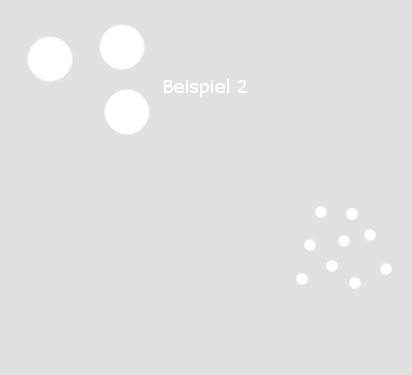
\includegraphics[width=0.50\textwidth]{./Bilder/bsp2.png}
	\caption{Beispiel 2 zum Einf�gen einer Grafik}
	\label{fig:bsp2}
\end{figure}

Praesent congue erat at massa. Sed cursus turpis vitae tortor. Donec posuere vulputate arcu. Phasellus accumsan cursus velit. Vestibulum ante ipsum primis in faucibus orci luctus et ultrices posuere cubilia Curae; Sed aliquam, nisi quis porttitor congue, elit erat euismod orci, ac placerat dolor lectus quis orci. Phasellus consectetuer vestibulum elit. Aenean tellus metus, bibendum sed, posuere ac, mattis non, nunc. Vestibulum fringilla pede sit amet augue. In turpis. Pellentesque posuere. Praesent turpis. Aenean posuere, tortor sed cursus feugiat, nunc augue blandit nunc, eu sollicitudin urna dolor sagittis lacus. Donec elit libero, sodales nec, volutpat a, suscipit non, turpis. Nullam sagittis. Suspendisse pulvinar, augue ac venenatis condimentum, sem libero volutpat nibh, nec pellentesque velit pede quis nunc. Vestibulum ante ipsum primis in faucibus orci luctus et ultrices posuere cubilia Curae; Fusce id purus. Ut varius tincidunt libero. Phasellus dolor. Maecenas vestibulum mollis diam. Pellentesque ut neque. Pellentesque habitant morbi tristique senectus et netus et malesuada fames ac turpis egestas. In dui magna, posuere eget, vestibulum et, tempor auctor, justo. In ac felis quis tortor malesuada pretium. Pellentesque auctor neque nec urna. Proin sapien ipsum, porta a, auctor quis, euismod ut, mi. Aenean viverra rhoncus pede. Pellentesque habitant morbi tristique senectus et netus et malesuada fames ac turpis egestas. Ut non enim eleifend felis pretium feugiat. Vivamus quis mi. Phasellus a est. Phasellus magna. In hac habitasse platea dictumst. Curabitur at lacus ac velit ornare lobortis. Curabitur a felis in nunc fringilla tristique (...)

\subsection{...}

 Sed cursus turpis vitae tortor. Donec posuere vulputate arcu. Phasellus accumsan cursus velit. Vestibulum ante ipsum primis in faucibus orci luctus et ultrices posuere cubilia Curae; Sed aliquam, nisi quis porttitor congue, elit erat euismod orci, ac placerat dolor lectus quis orci. Phasellus consectetuer vestibulum elit. Aenean tellus metus, bibendum sed, posuere ac, mattis non, nunc. Vestibulum fringilla pede sit amet augue. In turpis. Pellentesque posuere. Praesent turpis. Aenean posuere, tortor sed cursus feugiat, nunc augue blandit nunc, eu sollicitudin urna dolor sagittis lacus \cite{brink2005anfertigung}. Donec elit libero, sodales nec, volutpat a, suscipit non, turpis. Nullam sagittis. Suspendisse pulvinar, augue ac venenatis condimentum, sem libero volutpat nibh, nec pellentesque velit pede quis nunc. Vestibulum ante ipsum primis in faucibus orci luctus et ultrices posuere cubilia Curae; Fusce id purus. Ut varius tincidunt libero. Phasellus dolor. Maecenas vestibulum mollis diam. Pellentesque ut neque. Pellentesque habitant morbi tristique senectus et netus et malesuada fames ac turpis egestas. In dui magna, posuere eget, vestibulum et, tempor auctor, justo. In ac felis quis tortor malesuada pretium. Pellentesque auctor neque nec urna. Proin sapien ipsum, porta a, auctor quis, euismod ut, mi. Aenean viverra rhoncus pede. Pellentesque habitant morbi tristique senectus et netus et malesuada fames ac turpis egestas. Ut non enim eleifend felis pretium feugiat. Vivamus quis mi. Phasellus a est. Phasellus magna. In hac habitasse platea dictumst. Curabitur at lacus ac velit ornare lobortis. Curabitur a felis in nunc fringilla tristique. Vestibulum volutpat pretium libero. Cras id dui. Aenean ut eros et nisl sagittis vestibulum. Nullam nulla eros, ultricies sit amet, 
		\clearpage{\pagestyle{empty}\cleardoublepage}
    \chapter{Model}

Lorem ipsum dolor sit amet, consectetuer adipiscing elit. Aenean commodo ligula eget dolor. Aenean massa. Cum sociis natoque penatibus et magnis dis parturient montes, nascetur ridiculus mus. Donec quam felis, ultricies nec, pellentesque eu, pretium quis, sem. Nulla consequat massa quis enim. Donec pede justo, fringilla vel, aliquet nec, vulputate eget, arcu. In enim justo, rhoncus ut, imperdiet a, venenatis vitae, justo. Nullam dictum felis eu pede mollis pretium. Integer tincidunt. Cras dapibus. Vivamus elementum semper nisi. Aenean vulputate eleifend tellus. Aenean leo ligula, porttitor eu, consequat vitae, eleifend ac, enim. Aliquam lorem ante, dapibus in, viverra quis, feugiat a, tellus. Phasellus viverra nulla ut metus varius laoreet. Quisque rutrum. Aenean imperdiet. Etiam ultricies nisi vel augue. Curabitur ullamcorper ultricies nisi. Nam eget dui. Etiam rhoncus. Maecenas tempus, tellus eget condimentum rhoncus, sem quam semper libero, sit amet adipiscing sem neque sed ipsum. Nam quam nunc, blandit vel, luctus pulvinar, hendrerit id, lorem. Maecenas nec odio et ante tincidunt tempus. Donec vitae sapien ut libero venenatis faucibus. Nullam quis ante \cite{gopen1990science}.

\section{...}

 Etiam sit amet orci eget eros faucibus tincidunt. Duis leo. Sed fringilla mauris sit amet nibh. Donec sodales sagittis magna. Sed consequat, leo eget bibendum sodales, augue velit cursus nunc, quis gravida magna mi a libero. Fusce vulputate eleifend sapien. Vestibulum purus quam, scelerisque ut, mollis sed, nonummy id, metus. Nullam accumsan lorem in dui. Cras ultricies mi eu turpis hendrerit fringilla. Vestibulum ante ipsum primis in faucibus orci luctus et ultrices posuere cubilia Curae; In ac dui quis mi consectetuer lacinia. Nam pretium turpis et arcu. Duis arcu tortor, suscipit eget, imperdiet nec, imperdiet iaculis, ipsum. Sed aliquam ultrices mauris. Integer ante arcu, accumsan a, consectetuer eget, posuere ut, mauris. Praesent adipiscing. Phasellus ullamcorper ipsum rutrum nunc. Nunc nonummy metus. Vestibulum volutpat pretium libero. Cras id dui. Aenean ut eros et nisl sagittis vestibulum. Nullam nulla eros, ultricies sit amet, nonummy id, imperdiet feugiat, pede. Sed lectus. Donec mollis hendrerit risus. Phasellus nec sem in justo pellentesque facilisis. Etiam imperdiet imperdiet orci. Nunc nec neque. Phasellus leo dolor, tempus non, auctor et, hendrerit quis, nisi. Curabitur ligula sapien, tincidunt non, euismod vitae, posuere imperdiet, leo. Maecenas malesuada. 
\begin{figure}
	\centering
		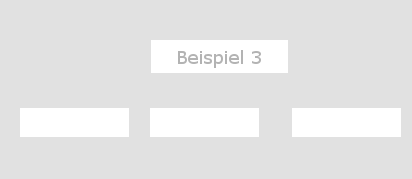
\includegraphics{./Bilder/bsp3.png}
	\caption{Beispiel 3 zum Einf�gen einer Grafik}
	\label{fig:bsp3}
\end{figure}
 
Praesent congue erat at massa. Sed cursus turpis vitae tortor. Donec posuere vulputate arcu. Phasellus accumsan cursus velit. Vestibulum ante ipsum primis in faucibus orci luctus et ultrices posuere cubilia Curae; Sed aliquam, nisi quis porttitor congue, elit erat euismod orci, ac placerat dolor lectus quis orci. Phasellus consectetuer vestibulum elit. Aenean tellus metus, bibendum sed, posuere ac, mattis non, nunc. Vestibulum fringilla pede sit amet augue. In turpis. Pellentesque posuere. Praesent turpis. Aenean posuere, tortor sed cursus feugiat, nunc augue blandit nunc, eu sollicitudin urna dolor sagittis lacus. Donec elit libero, sodales nec, volutpat a, suscipit non, turpis. Nullam sagittis. Suspendisse pulvinar, augue ac venenatis condimentum, sem libero volutpat nibh, nec pellentesque velit pede quis nunc. Vestibulum ante ipsum primis in faucibus orci luctus et ultrices posuere cubilia Curae; Fusce id purus. Ut varius tincidunt libero. Phasellus dolor. 
 
\begin{table}[bp]
	\centering
	\caption{Beispiel 2 zum Einf�gen einer Tabelle}
		\begin{tabular}{| c c c |}
		\hline
		\textbf{Taxonomie} & \textbf{Anzahl} & \textbf{Rohdatenwerte}\\ \hline \hline
             Verstorben & 104             &(verstorben)\\ \hline
      Pflegeheim       & 88              & (geht in station�re Einrichtung),(ist im Heim),...  \\ \hline 
Genesen&77&(genesen),(Wunde abgeheilt),(Wunde verheilt)\\ \hline
	\end{tabular}

\label{tab:Betreuungsende}
\end{table} 

Maecenas vestibulum mollis diam. Pellentesque ut neque. Pellentesque habitant morbi tristique senectus et netus et malesuada fames ac turpis egestas. In dui magna, posuere eget, vestibulum et, tempor auctor, justo. In ac felis quis tortor malesuada pretium. Pellentesque auctor neque nec urna. Proin sapien ipsum, porta a, auctor quis, euismod ut, mi. Aenean viverra rhoncus pede. Pellentesque habitant morbi tristique senectus et netus et malesuada fames ac turpis egestas. Ut non enim eleifend felis pretium feugiat. Vivamus quis mi. Phasellus a est. Phasellus magna. In hac habitasse platea dictumst. Curabitur at lacus ac velit ornare lobortis. Curabitur a felis in nunc fringilla tristique. Lorem ipsum dolor sit amet, consectetuer adipiscing elit. Aenean commodo ligula eget dolor. Aenean massa. Cum sociis natoque penatibus et magnis dis parturient montes, nascetur ridiculus mus. Donec quam felis, ultricies nec, pellentesque eu, pretium quis, sem. Nulla consequat massa quis enim. Donec pede justo, fringilla vel, aliquet nec, vulputate eget, arcu. In enim justo, rhoncus ut, imperdiet a, venenatis vitae, justo. Nullam dictum felis eu pede mollis pretium. Integer tincidunt. Cras dapibus. Vivamus elementum semper nisi. Aenean vulputate eleifend tellus. Aenean leo ligula, porttitor eu, consequat vitae, eleifend ac, enim. Aliquam lorem ante, dapibus in, viverra quis, feugiat a, tellus. Phasellus viverra nulla ut metus varius laoreet. Quisque rutrum. Aenean imperdiet. Etiam ultricies nisi vel augue. Curabitur ullamcorper ultricies nisi. Nam eget dui. Etiam rhoncus (...)

\section{...}

Maecenas tempus, tellus eget condimentum rhoncus, sem quam semper libero, sit amet adipiscing sem neque sed ipsum. Nam quam nunc, blandit vel, luctus pulvinar, hendrerit id, lorem. Maecenas nec odio et ante tincidunt tempus. Donec vitae sapien ut libero venenatis faucibus. Nullam quis ante. Etiam sit amet orci eget eros faucibus tincidunt. Duis leo. Sed fringilla mauris sit amet nibh. Donec sodales sagittis magna. Sed consequat, leo eget bibendum sodales, augue velit cursus nunc, quis gravida magna mi a libero. Fusce vulputate eleifend sapien. Vestibulum purus quam, scelerisque ut, mollis sed, nonummy id, metus. Nullam accumsan lorem in dui. Cras ultricies mi eu turpis hendrerit fringilla. Vestibulum ante ipsum primis in faucibus orci luctus et ultrices posuere cubilia Curae; In ac dui quis mi consectetuer lacinia. Nam pretium turpis et arcu. Duis arcu tortor, suscipit eget, imperdiet nec, imperdiet iaculis, ipsum. Sed aliquam ultrices mauris. Integer ante arcu, accumsan a, consectetuer eget, posuere ut, mauris. Praesent adipiscing. Phasellus ullamcorper ipsum rutrum nunc. Nunc nonummy metus. Vestibulum volutpat pretium libero. Cras id dui. Aenean ut eros et nisl sagittis vestibulum. Nullam nulla eros, ultricies sit amet, nonummy id, imperdiet feugiat, pede. Sed lectus. Donec mollis hendrerit risus. Phasellus nec sem in justo pellentesque facilisis. Etiam imperdiet imperdiet orci. Nunc nec neque. Phasellus leo dolor, tempus non, auctor et, hendrerit quis, nisi. Curabitur ligula sapien, tincidunt non, euismod vitae, posuere imperdiet, leo. Maecenas malesuada. Praesent congue erat at massa. Sed cursus turpis vitae tortor. Donec posuere vulputate arcu. Phasellus accumsan cursus velit. Vestibulum ante ipsum primis in faucibus orci luctus et ultrices posuere cubilia Curae; Sed aliquam, nisi quis porttitor congue, elit erat euismod orci, ac placerat dolor lectus quis orci. Phasellus consectetuer vestibulum elit. Aenean tellus metus, bibendum sed, posuere ac, mattis non, nunc. Vestibulum fringilla pede sit amet augue. In turpis. Pellentesque posuere. Praesent turpis. Aenean posuere, tortor sed cursus feugiat, nunc augue blandit nunc, eu sollicitudin urna dolor sagittis lacus. Donec elit libero, sodales nec, volutpat a, suscipit non, turpis. Nullam sagittis. Suspendisse pulvinar, augue ac venenatis condimentum, sem libero volutpat nibh, nec pellentesque velit pede quis nunc. Vestibulum ante ipsum primis in faucibus orci luctus et ultrices posuere cubilia Curae; Fusce id purus. Ut varius tincidunt libero. Phasellus dolor. Maecenas vestibulum mollis diam. Pellentesque ut neque. Pellentesque habitant morbi tristique senectus et netus et malesuada fames ac turpis egestas. In dui magna, posuere eget, vestibulum et, tempor auctor, justo. In ac felis quis tortor malesuada pretium. Pellentesque auctor neque nec urna. Proin sapien ipsum, porta a, auctor quis, euismod ut, mi. Aenean viverra rhoncus pede. Pellentesque habitant morbi tristique senectus et netus et malesuada fames ac turpis egestas. Ut non enim eleifend felis pretium feugiat. Vivamus quis mi. Phasellus a est. Phasellus magna. In hac habitasse platea dictumst. Curabitur at lacus ac velit ornare lobortis. Curabitur a felis in nunc fringilla tristique. Lorem ipsum dolor sit amet, consectetuer adipiscing elit. Aenean commodo ligula eget dolor. Aenean massa. Cum sociis natoque penatibus et magnis dis parturient montes, nascetur ridiculus mus. Donec quam felis, ultricies nec, pellentesque eu, pretium quis, sem. Nulla consequat massa quis enim. Donec pede justo, fringilla vel, aliquet nec, vulputate eget, arcu. In enim justo, rhoncus ut, imperdiet a, venenatis vitae, justo. Nullam dictum felis eu pede mollis pretium. Integer tincidunt. Cras dapibus. Vivamus elementum semper nisi. Aenean vulputate eleifend tellus. Aenean leo ligula, porttitor eu, consequat vitae, eleifend ac, enim. Aliquam lorem ante, dapibus in, viverra quis, feugiat a, tellus. Phasellus viverra nulla ut metus varius laoreet. Quisque rutrum. Aenean imperdiet. Etiam ultricies nisi vel augue. Curabitur ullamcorper ultricies nisi. Nam eget dui. Etiam rhoncus. Maecenas tempus, tellus eget condimentum rhoncus, sem quam semper libero, sit amet adipiscing sem neque sed ipsum. Nam quam nunc, blandit vel, luctus pulvinar, hendrerit id, lorem. Maecenas nec odio et ante tincidunt tempus. Donec vitae sapien ut libero venenatis faucibus. Nullam quis ante. Etiam sit amet orci eget eros faucibus tincidunt. Duis leo. Sed fringilla mauris sit amet nibh. Donec sodales sagittis magna. Sed consequat, leo eget bibendum sodales, augue velit cursus nunc, quis gravida magna mi a libero. Fusce vulputate eleifend sapien. Vestibulum purus quam, scelerisque ut, mollis sed, nonummy id, metus. Nullam accumsan lorem in dui. Cras ultricies mi eu turpis hendrerit fringilla. Vestibulum ante ipsum primis in faucibus orci luctus et ultrices posuere cubilia Curae; In ac dui quis mi consectetuer lacinia. Nam pretium turpis et arcu. Duis arcu tortor, suscipit eget, imperdiet nec, imperdiet iaculis, ipsum. Sed aliquam ultrices mauris. Integer ante arcu, accumsan a, consectetuer eget, posuere ut, mauris. Praesent adipiscing. Phasellus ullamcorper ipsum rutrum nunc. Nunc nonummy metus. Vestibulum volutpat pretium libero. Cras id dui. Aenean ut eros et nisl sagittis vestibulum. Nullam nulla eros, ultricies sit amet, nonummy id, imperdiet feugiat, pede. Sed lectus. Donec mollis hendrerit risus. Phasellus nec sem in justo pellentesque facilisis. Etiam imperdiet imperdiet orci. Nunc nec neque. Phasellus leo dolor, tempus non, auctor et, hendrerit quis, nisi. Curabitur ligula sapien, tincidunt non, euismod vitae, posuere imperdiet, leo. Maecenas malesuada. Praesent congue erat at massa. Sed cursus turpis vitae tortor. Donec posuere vulputate arcu. Phasellus accumsan cursus velit. Vestibulum ante ipsum primis in faucibus orci luctus et ultrices posuere cubilia Curae; Sed aliquam, nisi quis porttitor congue, elit erat euismod orci, ac placerat dolor lectus quis orci. Phasellus consectetuer vestibulum elit. Aenean tellus metus, bibendum sed, posuere ac, mattis non, nunc. Vestibulum fringilla pede sit amet augue. In turpis. Pellentesque posuere. Praesent turpis. Aenean posuere, tortor sed cursus feugiat, nunc augue blandit nunc, eu sollicitudin urna dolor sagittis lacus. Donec elit libero, sodales nec, volutpat a, suscipit non, turpis.


\section{...}

Nullam sagittis (...) 
    \clearpage{\pagestyle{empty}\cleardoublepage}
    \chapter{Results/Analysis}

Lorem ipsum dolor sit amet, consectetuer adipiscing elit. Aenean commodo ligula eget dolor. Aenean massa. Cum sociis natoque penatibus et magnis dis parturient montes, nascetur ridiculus mus. Donec quam felis, ultricies nec, pellentesque eu, pretium quis, sem. Nulla consequat massa quis enim. Donec pede justo, fringilla vel, aliquet nec, vulputate eget, arcu. In enim justo, rhoncus ut, imperdiet a, venenatis vitae, justo. Nullam dictum felis eu pede mollis pretium. Integer tincidunt. Cras dapibus. Vivamus elementum semper nisi. Aenean vulputate eleifend tellus. Aenean leo ligula, porttitor eu, consequat vitae, eleifend ac, enim. Aliquam lorem ante, dapibus in, viverra quis, feugiat a, tellus. Phasellus viverra nulla ut metus varius laoreet. Quisque rutrum. Aenean imperdiet. Etiam ultricies nisi vel augue. Curabitur ullamcorper ultricies nisi. Nam eget dui. Etiam rhoncus. Maecenas tempus, tellus eget condimentum rhoncus, sem quam semper libero, sit amet adipiscing sem neque sed ipsum. Nam quam nunc, blandit vel, luctus pulvinar, hendrerit id, lorem. Maecenas nec odio et ante tincidunt tempus. Donec vitae sapien ut libero venenatis faucibus. Nullam quis ante.

\section{...}

 Etiam sit amet orci eget eros faucibus tincidunt. Duis leo. Sed fringilla mauris sit amet nibh. Donec sodales sagittis magna. Sed consequat, leo eget bibendum sodales, augue velit cursus nunc, quis gravida magna mi a libero. Fusce vulputate eleifend sapien. Vestibulum purus quam, scelerisque ut, mollis sed, nonummy id, metus. Nullam accumsan lorem in dui. Cras ultricies mi eu turpis hendrerit fringilla. Vestibulum ante ipsum primis in faucibus orci luctus et ultrices posuere cubilia Curae; In ac dui quis mi consectetuer lacinia. Nam pretium turpis et arcu. Duis arcu tortor, suscipit eget, imperdiet nec, imperdiet iaculis, ipsum. Sed aliquam ultrices mauris. Integer ante arcu, accumsan a, consectetuer eget, posuere ut, mauris. Praesent adipiscing. Phasellus ullamcorper ipsum rutrum nunc. Nunc nonummy metus. Vestibulum volutpat pretium libero. Cras id dui. Aenean ut eros et nisl sagittis vestibulum. Nullam nulla eros, ultricies sit amet, nonummy id, imperdiet feugiat, pede. Sed lectus. Donec mollis hendrerit risus. Phasellus nec sem in justo pellentesque facilisis. Etiam imperdiet imperdiet orci. Nunc nec neque. Phasellus leo dolor, tempus non, auctor et, hendrerit quis, nisi. Curabitur ligula sapien, tincidunt non, euismod vitae, posuere imperdiet, leo. Maecenas malesuada. Praesent congue erat at massa. Sed cursus turpis vitae tortor. Donec posuere vulputate arcu. Phasellus accumsan cursus velit. Vestibulum ante ipsum primis in faucibus orci luctus et ultrices posuere cubilia Curae; Sed aliquam, nisi quis porttitor congue, elit erat euismod orci, ac placerat dolor lectus quis orci. Phasellus consectetuer vestibulum elit. Aenean tellus metus, bibendum sed, posuere ac, mattis non, nunc. Vestibulum fringilla pede sit amet augue. In turpis. Pellentesque posuere. Praesent turpis. Aenean posuere, tortor sed cursus feugiat, nunc augue blandit nunc, eu sollicitudin urna dolor sagittis lacus. Donec elit libero, sodales nec, volutpat a, suscipit non, turpis. Nullam sagittis. Suspendisse pulvinar, augue ac venenatis condimentum, sem libero volutpat nibh, nec pellentesque velit pede quis nunc. Vestibulum ante ipsum primis in faucibus orci luctus et ultrices posuere cubilia Curae; Fusce id purus. Ut varius tincidunt libero. Phasellus dolor. Maecenas vestibulum mollis diam. Pellentesque ut neque. Pellentesque habitant morbi tristique senectus et netus et malesuada fames ac turpis egestas. In dui magna, posuere eget, vestibulum et, tempor auctor, justo. In ac felis quis tortor malesuada pretium. Pellentesque auctor neque nec urna. Proin sapien ipsum, porta a, auctor quis, euismod ut, mi. Aenean viverra rhoncus pede. Pellentesque habitant morbi tristique senectus et netus et malesuada fames ac turpis egestas. Ut non enim eleifend felis pretium feugiat. Vivamus quis mi. Phasellus a est. Phasellus magna. In hac habitasse platea dictumst. Curabitur at lacus ac velit ornare lobortis. Curabitur a felis in nunc fringilla tristique. Lorem ipsum dolor sit amet, consectetuer adipiscing elit. Aenean commodo ligula eget dolor. Aenean massa. Cum sociis natoque penatibus et magnis dis parturient montes, nascetur ridiculus mus. Donec quam felis, ultricies nec, pellentesque eu, pretium quis, sem. Nulla consequat massa quis enim. Donec pede justo, fringilla vel, aliquet nec, vulputate eget, arcu. In enim justo, rhoncus ut, imperdiet a, venenatis vitae, justo. Nullam dictum felis eu pede mollis pretium. Integer tincidunt. Cras dapibus. Vivamus elementum semper nisi. Aenean vulputate eleifend tellus. Aenean leo ligula, porttitor eu, consequat vitae, eleifend ac, enim. Aliquam lorem ante, dapibus in, viverra quis, feugiat a, tellus. Phasellus viverra nulla ut metus varius laoreet. Quisque rutrum. Aenean imperdiet. Etiam ultricies nisi vel augue. Curabitur ullamcorper ultricies nisi. Nam eget dui. Etiam rhoncus...

\section{...}

Maecenas tempus, tellus eget condimentum rhoncus, sem quam semper libero, sit amet adipiscing sem neque sed ipsum. Nam quam nunc, blandit vel, luctus pulvinar, hendrerit id, lorem. Maecenas nec odio et ante tincidunt tempus. Donec vitae sapien ut libero venenatis faucibus. Nullam quis ante. Etiam sit amet orci eget eros faucibus tincidunt. Duis leo. Sed fringilla mauris sit amet nibh. Donec sodales sagittis magna. Sed consequat, leo eget bibendum sodales, augue velit cursus nunc, quis gravida magna mi a libero. Fusce vulputate eleifend sapien. Vestibulum purus quam, scelerisque ut, mollis sed, nonummy id, metus. Nullam accumsan lorem in dui. Cras ultricies mi eu turpis hendrerit fringilla. Vestibulum ante ipsum primis in faucibus orci luctus et ultrices posuere cubilia Curae; In ac dui quis mi consectetuer lacinia. Nam pretium turpis et arcu. Duis arcu tortor, suscipit eget, imperdiet nec, imperdiet iaculis, ipsum. Sed aliquam ultrices mauris. Integer ante arcu, accumsan a, consectetuer eget, posuere ut, mauris. Praesent adipiscing. Phasellus ullamcorper ipsum rutrum nunc. Nunc nonummy metus. Vestibulum volutpat pretium libero. Cras id dui. Aenean ut eros et nisl sagittis vestibulum. Nullam nulla eros, ultricies sit amet, nonummy id, imperdiet feugiat, pede. Sed lectus. Donec mollis hendrerit risus. Phasellus nec sem in justo pellentesque facilisis. Etiam imperdiet imperdiet orci. Nunc nec neque. Phasellus leo dolor, tempus non, auctor et, hendrerit quis, nisi. Curabitur ligula sapien, tincidunt non, euismod vitae, posuere imperdiet, leo. Maecenas malesuada. Praesent congue erat at massa. Sed cursus turpis vitae tortor. Donec posuere vulputate arcu. Phasellus accumsan cursus velit. Vestibulum ante ipsum primis in faucibus orci luctus et ultrices posuere cubilia Curae; Sed aliquam, nisi quis porttitor congue, elit erat euismod orci, ac placerat dolor lectus quis orci. Phasellus consectetuer vestibulum elit. Aenean tellus metus, bibendum sed, posuere ac, mattis non, nunc. Vestibulum fringilla pede sit amet augue. In turpis. Pellentesque posuere. Praesent turpis. Aenean posuere, tortor sed cursus feugiat, nunc augue blandit nunc, eu sollicitudin urna dolor sagittis lacus. Donec elit libero, sodales nec, volutpat a, suscipit non, turpis. Nullam sagittis. Suspendisse pulvinar, augue ac venenatis condimentum, sem libero volutpat nibh, nec pellentesque velit pede quis nunc. Vestibulum ante ipsum primis in faucibus orci luctus et ultrices posuere cubilia Curae; Fusce id purus. Ut varius tincidunt libero. Phasellus dolor. Maecenas vestibulum mollis diam. Pellentesque ut neque. Pellentesque habitant morbi tristique senectus et netus et malesuada fames ac turpis egestas. In dui magna, posuere eget, vestibulum et, tempor auctor, justo. In ac felis quis tortor malesuada pretium. Pellentesque auctor neque nec urna. Proin sapien ipsum, porta a, auctor quis, euismod ut, mi. Aenean viverra rhoncus pede. Pellentesque habitant morbi tristique senectus et netus et malesuada fames ac turpis egestas. Ut non enim eleifend felis pretium feugiat. Vivamus quis mi. Phasellus a est. Phasellus magna. In hac habitasse platea dictumst. Curabitur at lacus ac velit ornare lobortis. Curabitur a felis in nunc fringilla tristique. Lorem ipsum dolor sit amet, consectetuer adipiscing elit. Aenean commodo ligula eget dolor. Aenean massa. Cum sociis natoque penatibus et magnis dis parturient montes, nascetur ridiculus mus. Donec quam felis, ultricies nec, pellentesque eu, pretium quis, sem. Nulla consequat massa quis enim. Donec pede justo, fringilla vel, aliquet nec, vulputate eget, arcu. In enim justo, rhoncus ut, imperdiet a, venenatis vitae, justo. Nullam dictum felis eu pede mollis pretium. Integer tincidunt. Cras dapibus. Vivamus elementum semper nisi. Aenean vulputate eleifend tellus. Aenean leo ligula, porttitor eu, consequat vitae, eleifend ac, enim. Aliquam lorem ante, dapibus in, viverra quis, feugiat a, tellus. Phasellus viverra nulla ut metus varius laoreet. Quisque rutrum. Aenean imperdiet. Etiam ultricies nisi vel augue. Curabitur ullamcorper ultricies nisi. Nam eget dui. Etiam rhoncus. Maecenas tempus, tellus eget condimentum rhoncus, sem quam semper libero, sit amet adipiscing sem neque sed ipsum. Nam quam nunc, blandit vel, luctus pulvinar, hendrerit id, lorem. Maecenas nec odio et ante tincidunt tempus. Donec vitae sapien ut libero venenatis faucibus. Nullam quis ante. Etiam sit amet orci eget eros faucibus tincidunt. Duis leo. Sed fringilla mauris sit amet nibh. Donec sodales sagittis magna. Sed consequat, leo eget bibendum sodales, augue velit cursus nunc, quis gravida magna mi a libero. Fusce vulputate eleifend sapien. Vestibulum purus quam, scelerisque ut, mollis sed, nonummy id, metus. Nullam accumsan lorem in dui. Cras ultricies mi eu turpis hendrerit fringilla. Vestibulum ante ipsum primis in faucibus orci luctus et ultrices posuere cubilia Curae; In ac dui quis mi consectetuer lacinia. Nam pretium turpis et arcu. Duis arcu tortor, suscipit eget, imperdiet nec, imperdiet iaculis, ipsum. Sed aliquam ultrices mauris. Integer ante arcu, accumsan a, consectetuer eget, posuere ut, mauris. Praesent adipiscing. Phasellus ullamcorper ipsum rutrum nunc. Nunc nonummy metus. Vestibulum volutpat pretium libero. Cras id dui. Aenean ut eros et nisl sagittis vestibulum. Nullam nulla eros, ultricies sit amet, nonummy id, imperdiet feugiat, pede. Sed lectus. Donec mollis hendrerit risus. Phasellus nec sem in justo pellentesque facilisis. Etiam imperdiet imperdiet orci. Nunc nec neque. Phasellus leo dolor, tempus non, auctor et, hendrerit quis, nisi. Curabitur ligula sapien, tincidunt non, euismod vitae, posuere imperdiet, leo. Maecenas malesuada. Praesent congue erat at massa. Sed cursus turpis vitae tortor. Donec posuere vulputate arcu. Phasellus accumsan cursus velit. Vestibulum ante ipsum primis in faucibus orci luctus et ultrices posuere cubilia Curae; Sed aliquam, nisi quis porttitor congue, elit erat euismod orci, ac placerat dolor lectus quis orci. Phasellus consectetuer vestibulum elit. Aenean tellus metus, bibendum sed, posuere ac, mattis non, nunc. Vestibulum fringilla pede sit amet augue. In turpis. Pellentesque posuere. Praesent turpis. Aenean posuere, tortor sed cursus feugiat, nunc augue blandit nunc, eu sollicitudin urna dolor sagittis lacus. Donec elit libero, sodales nec, volutpat a, suscipit non, turpis.


\section{...}

Nullam sagittis ... 
    \clearpage{\pagestyle{empty}\cleardoublepage}
    \chapter{Conclusion and Outlook}

(...)
    \clearpage{\pagestyle{empty}\cleardoublepage}

% -----------------------------------
\backmatter 
\bibliographystyle{apacite}				% by natbib in german
\bibliography{./literature/sources}		% including literature sources
\newpage
\thispagestyle{empty}

\begin{large}

\vspace*{2cm}

\noindent
I declare that I have authored this thesis independently, that I have not used other than the declared sources / resources, and that I have explicitly marked all material which has been quoted either literally or by content from the used sources.

\vspace{2cm}

\noindent
Berlin, February 1, 2042
\vspace{3cm}

\hspace*{7cm}%
\dotfill\\
\hspace*{8.5cm}%
\textit{(Signature of the author)}

\end{large}
 			% % statutory declaration - "`Eidesstattliche Erkl�rung"'

\end{document}